\section{Discussion}\label{sec:discussion}
In this section, we will discuss the design space and reflect about some of the design decisions of our work. We relate 
our language to traits, Java interfaces as well as other languages. Furthermore, we discuss
ways to improve our work.

\subsection{Abstract Methods}

Abstract methods are one of the key features in most general OO languages. For example, Java interfaces were designed
to include only method declarations, and those abstract methods can be implemented in a class body. 
The formal Featherweight Java model~\cite{Igarashi01FJ} does not include abstract methods because of the orthogonality
to the core calculus. In traits, the
similar idea is to use keywords like ``\textbf{require}'' for abstract method declarations~\cite{scharli03traits}.
Abstract methods provide a way to
delay the implementations to future subtypes. Using overriding, they also help to ``exclude'' existing implementations.

In our formalized calculus, however, abstract methods are not a completely orthogonal feature. The $\canInstantiate$ function
has to check whether an interface can be instantiated by looking at all the inherited branches and checking if each most specific method is abstract or not.

Our formalization has a simple form of abstract methods, which behave similarly to conventional methods with respect to conflicts.
Other languages may behave differently. 
For instance, in Java 8 when putting two identical abstract methods together by multiple inheritance, there is no conflict error. In Figure~\ref{fig:abstractdiamond}, we use italic $\emph{m}$ to denote abstract methods. In both cases, the Java compiler accepts the definition of $C$ and automatically merges the two inherited methods $m$ into a single one. \MIM{} behaves differently from Java in both cases.
In the triangle inheritance case (left), $C$ will have two distinct abstract methods corresponding to $A.m$ and $B.m$. 
In the diamond inheritance case, the definition of $C$ is rejected. 
There are two reasons for this difference in behaviour. Firstly, our formalization just treats abstract methods as concrete methods with an empty body, and that simplifies
the rules and proofs a lot. Secondly, and more importantly, we distinguish and treat differently conflicting methods, since they may represent different operations, even if they are abstract. Thus our model adopts a very conservative behavior rather than automatically merging 
methods by default (as done in many languages). 
Arguably, for the diamond case, as we have mentioned, it is actually an intentional conflict due to the same source $T$.
It is possible to change our model to account for other behaviors for abstract methods, but we view this as a mostly 
orthogonal change to our work, that should not affect the essence of the model presented here.

\begin{figure*}[t]
\saveSpaceFig
    % \nocaptionrule
    % \centering
    \centering
    \begin{minipage}[t]{0.45\textwidth}
        \centering
        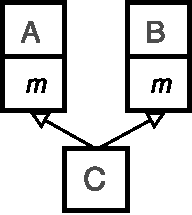
\includegraphics[width=1.6cm]{pics/P7.pdf}
    \end{minipage}
    \centering
    \hspace*{2pt}
    \begin{minipage}[t]{0.45\textwidth}
        \centering
        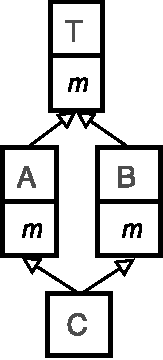
\includegraphics[width=1.4cm]{pics/P8.pdf}
    \end{minipage}  
    \caption{Triangle inheritance (left) and diamond inheritance (right) on abstract methods.}\label{fig:abstractdiamond}
\saveSpaceFig
\end{figure*}

\subsection{Orthogonal \& Non-Orthogonal Extensions}\label{sec:orthoext}
Our model is designed as a minimal calculus that focuses on resolving unintentional conflicts. Therefore, we have omitted a number of
common orthogonal features including primitive types, assignments, method overloading, covariant method return types, static dispatch, and so on.
Those features can, in principle, be modularly added to the model without breaking type soundness. For example, we present the additional syntax, typing and semantic rules of static invocation below as an extension:

\begin{mathpar}
    \begin{array}{llrl}
        \text{Expressions}  & e  & \Coloneqq & \ldots \; \mid \; e.J_0@J_1::m(\overline{e})
    \end{array} \\
    \tstaticinvk \\
    \sstaticinvk
\end{mathpar}
A static invocation $e.J_0@J_1::m(\overline{e})$ aims at finding the method $m$ in $J_0$ that hierarchically overrides $J_1$, thus $J_0[m\ \kwoverride\ J_1]$ is invoked. As shown in \textsc{(S-StaticInvk)}, static dispatch needs a receiver for the substitution of the ``$\kwthis$'' reference, so as to provide the latest implementations. In fact, static dispatch is common in OO programming, as it provides a shortcut to the reuse of old implementation easily, and super calls can also rely on this feature. For convenience we just make it simple above, whereas in languages like C++ or Java, the static or super invocations are more flexible, as they can climb the class hierarchy. 

One typical non-orthogonal extension to \MIM{} could be to have fields.
The design of \MIM{} can be viewed as a variant of Java 8 with default methods which allows for unintentional method conflicts.
Like Java interfaces and traits, state is forbidden in \MIM{}. There are some inheritance models that also account for fields, such as C++ that uses virtual inheritance~\cite{ellis1990annotated}. In our model, however, we can perhaps borrow the idea of \textit{interface-based programming}~\cite{classless}, which models state with abstract state operations. This can be realized by extending our current model with static methods and anonymous classes from Java. However such an extension requires more thought, so we leave it to future work.

\subsection{Loosening the Model: Reject Early or Reject Later?}\label{subsec:loosen}

\MIM{} rejects the following case of diamond inheritance:
\begin{lstlisting}
interface A { void m() {...} }
interface B extends A { void m() {...} }
interface C extends A { void m() {...} }
interface D extends B, C {}
\end{lstlisting}
Here both $B.m$ and $C.m$ override $A.m$, and D inherits
both conflicting methods without an explicit override. In this case automatically merging 
the two methods (to achieve diamond inheritance) is not possible, which is why many 
models (like traits and Java 8) reject such programs. Moreover, keeping the two 
method implementations in \lstinline|D| is problematic. 
In essence, hierarchical information is 
not helpful to disambiguate later method calls, since the two methods share 
the same origin (\lstinline|A.m|). 
Our calculus rejects such conflicts by the \textsc{(T-Intf)} rule, where $D$ is considered to be ill-formed. 
We believe that rejecting \lstinline|D| follows the principle of models like traits and Java 8 interfaces, 
where the language/type-system is meant to alert the programmer for a possible conflict early.

Nonetheless,
 C++ accepts the definition of $D$, but forbids later upcasts from $D$ to $A$ because of ambiguity. Our language is more conservative on definitions of interfaces compared to C++, but on the upside, upcasts are not rejected. We could also loosen the model to accept definitions such as \lstinline|D|, and perform ambiguity check on upcasts and other expressions. However, we would need to handle more cases than C++. For instance, in the above program assume that $B.m$ and $C.m$ are hierarchical overrides on $A$. Then such a case is still a diamond.

\begin{comment}
Another case is about the restriction on hierarchical overrides. In our language model there are two types of methods (though they share the same syntax): original methods and hierarchical overrides. We require that a hierarchical override should only override an original method. Yet from the idea of encapsulation and modularity on programs, we could also allow an override to work on another override, which forms a series of overrides.
\end{comment}

%\haoyuan{more. 1) Path Invocation, more generalized diamond inheritance: not clear; other method resolution techniques: no example; better code reuse with other kinds of method invocation: no example. }
